\chapter{Trabajo de investigación: Efectos Regionales} \label{3}

\section{Casos de estudio}
Para este primer trabajo, se seleccionaron 20 TG para identificar respuestas geomagnéticas regionales. La primera ventana de estudio abarca desde el 2003 hasta el 2018 para los casos de estudio cuyos datos de campo magnético local fueron proporcionados por el observatorio magnético de Teoloyucan (TEO). Para estudios más recientes por otro lado (a partir de enero del 2023), se están empleando datos de campo magnético de la estación magnética de Coeneo (COE), siendo 3 los eventos con los que se está trabajando por el momento. Ambos sitios se encuentran en una latitud geomagnética muy parecida ($\sim 28$). Mientras que TEO es operado por el Servicio Magnético adscrito al Instituto de Geofísica de la Universidad Nacional Autónoma de México, COE forma parte del reciente proyecto de la Red nacional de magnetómetros en México (REGMEX) liderado por el Dr. Pedro Corona Romero.
\vspace{1 em}

El criterio de selección de los casos de estudio se basó en considerar como base la respuesta geomagnética local (índices $K_{TEO}/K_{COE}$ y $\Delta H_{TEO}/\Delta_{COE}$). En el caso de los índices K, se consideraron aquellas TG con valores mayores a 6+, así como aquellos eventos donde $\Delta H$ esté por debajo de -120 nT. En la tabla \ref{table1:GS_descp} se proporcionan los detalles de los eventos:

\begin{table*}[h!]
\normalsize
\centering
    \caption{Casos de estudio: Número de evento, TG Fecha de inicio de la fase principal, Mínimo (Máximo) valor alcanzado durante los eventos para ${\rm Dst}$(${\rm K_P}$) y ${\rm \Delta H_{TEO}}$(${\rm K_{TEO}}$)}
    \label{table1:GS_descp}
\begin{tabular}{cccccc}
\hline
Evento & Inicio de & $^a {\rm Dst}$ mínimo
 & $^b{\rm \Delta H}$ mínimo
 & $^a{\rm K_p}$ & $^b {\rm K_{TEO}}$ \\
\#    & fase principal & [nT] & [nT] & máximo & máximo\\
\hline
1 & 2003/05/29 & -144 & -190 & 8+ & 9 \\ 
2 & 2003/10/14 & -85 & -126 & 7+ & 7- \\ 
3 & 2003/11/20 & -422 & -441 & 9- & 9 \\ 
4 & 2004/07/22 & -170 & -167 & 9- & 8+ \\ 
5 & 2004/08/30 & -129 & -154 & 7 & 7- \\ 
6 & 2004/11/08 & -374 & -398 & 9- & 9 \\ 
7 & 2005/05/15 & -247 & -206 & 8+ & 7 \\ 
8 & 2005/06/12 & -106 & -120 & 7+ & 6+ \\ 
9 & 2005/08/24 & -184 & -138 & 9- & 9- \\ 
10 & 2005/08/31 & -122 & -125 & 7 & 6+ \\ 
11 & 2006/08/19 & -79 & -131 & 6 & 7- \\ 
12 & 2006/12/14 & -162 & -247 & 8+ & 9 \\ 
13 & 2015/03/15 & -222 & -282 & 8 & 8- \\ 
14 & 2015/10/07 & -124 & -143 & 7+ & 7+ \\ 
15 & 2015/12/20 & -155 & -189 & 7- & 7 \\ 
16 & 2016/03/06 & -98 & -120 & 6 & 7 \\ 
17 & 2016/10/13 & -104 & -128 & 6+ & 6+ \\ 
18 & 2017/05/27 & -125 & 145 & 7 & 8 \\ 
19 & 2017/09/07 & -124 & -170 & 8+ & 8+ \\ 
20 & 2018/09/25 & -175 & -176 & 7+ & 7- \\ 
\hline
\multicolumn{6}{l}{Comentarios para la tabla.} \\
\multicolumn{6}{l}{$^a$ Dst y Kp fueron obtenidos de \href{http://isgi.unistra.fr/data_download.php}{International Service of Geomagnetic Indices (ISGI)}.}\\
\multicolumn{6}{l}{$^b$ Índices geomagnéticos regionales $\mathrm{\Delta H_{TEO}}$ and ${\rm K_{TEO}}$Fueron calculados por el Laboratorio Nacional} \\
\multicolumn{6}{l}{de Clima Espacial, usando observaciones de TEO.}    \end{tabular}
\end{table*}


\begin{table*}[h!]
\normalsize
\centering
    \caption{Casos de estudio: Número de evento, TG Fecha de inicio de la fase principal, Mínimo (Máximo) valor alcanzado durante los eventos para ${\rm SYM-H}$(${\rm K_P}$) y ${\rm \Delta H_{COE}}$(${\rm K_{COE}}$)}
    \label{table2:GS_descp}
\begin{tabular}{cccccc}
\hline
Evento & Inicio de & $^a {\rm SYM-H}$ mínimo
 & $^b{\rm \Delta H}$ mínimo
 & $^a{\rm K_p}$ & $^b {\rm K_{COE}}$ \\
\#    & fase principal & [nT] & [nT] & máximo & máximo\\
\hline
21 & 2023/02/26 & -144 & -190 & 8+ & 9 \\ 
22 & 2023/03/23 & -85 & -126 & 7+ & 7- \\ 
23 & 2023/04/23 & -422 & -441 & 9- & 9 \\ 
\hline
\multicolumn{6}{l}{Comentarios para la tabla.} \\
\multicolumn{6}{l}{$^a$ SYM-H y Kp fueron obtenidos de \href{http://isgi.unistra.fr/data_download.php}{International Service of Geomagnetic Indices (ISGI)}.}\\
\multicolumn{6}{l}{$^b$ Índices geomagnéticos regionales $\mathrm{\Delta H_{COE}}$ and ${\rm K_{COE}}$Fueron calculados por el Laboratorio Nacional} \\
\multicolumn{6}{l}{de Clima Espacial, usando observaciones de COE.}    \end{tabular}
\end{table*}

\section{Diferencias en la respuesta geomagnética} \label{respuesta_dif}

La hipótesis considerada para este trabajo es que pueden haber diferencias significativas observadas entre los índices regionales y planetarios, las cuales se deben a manifestaciones geomagnéticas. Para abordar esto, se comparó directamente ${\rm Dst}$ con $\Delta H_{\rm TEO}$ para los casos analizados. La Figura \ref{fig:disp} ilustra esta comparación, mostrando la respuesta geomagnética regional en el eje vertical, con su contra-parte planetaria en el eje horizontal. La gráfica revela dos diferentes tendencias en la distribución de los datos:

\begin{itemize}
    \item Para eventos con ${\rm Dst} \ge {\rm -100}$ nT, los datos puntuales se encuentran cercanos a la linea de identidad (línea negra diagonal).
    \item Para eventos con ${\rm Dst} < {\rm -100}$ nT (región sombreada verde), los datos se desvían de la linea de identidad.
\end{itemize}

Estas tendencias son consistentes con los índices de correlación, siendo $R^2=0.77$ para el primer caso, mientras que para el segundo $R^2=0.42$. Una mayor dispersión en conjunto con una disminución en la correlación, indica variaciones significativas en la respuesta regional con respecto de la planetaria. De esta forma, el siguiente paso es el de identificar los mecanismos físicos que puedan dar origen a estas variaciones regionales. De acuerdo con estudios realizados en México por \cite{dramaria_1, dramaria7, P-corona1, P-corona2}, estas variaciones pueden tener su origen debido a actividad ionosférica asociada a la TG. Por otro lado, según \cite{ddyn2005, angeoddyn, amorymazaudier_2017, amory2020_filtros} se relacionan con corrientes ionosféricas \ref{diono}

\begin{figure}
    \centering
     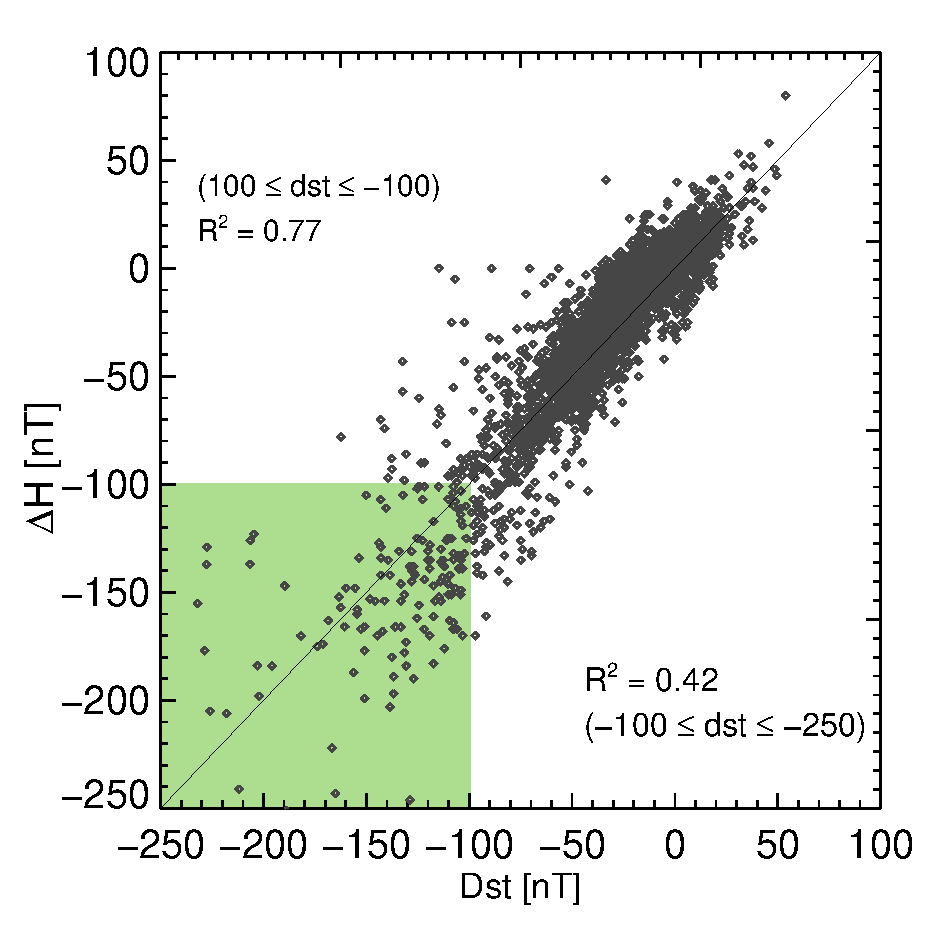
\includegraphics[width=0.7\textwidth]{Images/dispersion_general_dst.eps}
      \caption{Gráfica de dispersión de $\Delta$H (eje vertical) con respecto a Dst (eje horizontal) para todos los eventos TG. La región verde representa un umbral de -100 nT en que fue calculado $R^2$.}
       \label{fig:disp}
\end{figure}


\section{Identificación de firmas magnéticas}

Los valores locales del CMT resultan del efecto combinado de diferentes fuentes que contribuyen al campo total \cite{iaga_guide, 1969intro_to_iono_p, l_handbook_geof_sw_Geom_field, baseline_Gjerloev, vanKampt}. Estas fuentes contribuyen a la componente H del CMT local, lo cual puede expresarse como:

\begin{equation}
    \label{eq:1}
        H = H_{SQ} + H_0 + D_{M} + D_{I},
\end{equation}

donde $H_{SQ}$ representa la variación diurna derivada de los días quietos locales \cite{vanKampt}, mientras que $H_0$ representa las variaciones día a día \cite{baseline_Gjerloev}. Los últimos términos representan las perturbaciones asociadas con la TG y representan la contribución de las corrientes magnetosféricas e ionosféricas respectivamente \cite{ddyn2005, angeoddyn}. La contribución de $D_M$ para latitudes geomagnéticas medias y bajas puede aproximarse de la siguiente forma $Dst \cdot \cos(\lambda)$, donde $\lambda$ es la latitud geomagnética de donde fueron tomados los datos \cite{amorymazaudier_2017}. 
\vspace{1 em}

Considerando lo mencionado en secciones anteriores, la contribución de interés es la asociada con mecanismos ionosféricos o $D_I$, por lo que el siguiente paso es simplemente aislarlo del resto de contribuciones magnéticas. Para ello, a partir de la expresión \ref{eq:1}:

\begin{equation}
\label{eq:diono}
   D_{I} \approx H -(H_{SQ} +  H_0 + Dst \cdot cos(\lambda)).
\end{equation}

Además, de acuerdo con \cite{ddyn2005, angeoddyn}, en latitudes medias y bajas, $D_I$ es la suma de las firmas magnéticas de CPP2 y CDP:
\begin{equation}
\label{eq:diono_explicit}
   D_{I} = H_{Ddyn} + H_{DP2} + H_{otras},
\end{equation}

donde $H_{otras}$ se refiere a cualquier otra perturbación de origen ionosférico, diferente de \emph{Ddyn} y \emph{DP2}.
\vspace{1 em}

Para aislar de forma efectiva las firmas magnéticas atribuidas a $H_{Ddyn}$ y a $H_{DP2}$ en las ecuaciones \ref{eq:diono} y \ref{eq:diono_explicit}, se empleó de forma inicial un filtro de frecuencias para analizar $D_I$ \cite{amory2020_filtros}. Estos filtros fueron diseñados de acuerdo con los rangos de frecuencias (periodos) en que las corrientes \emph{Ddyn} y \emph{DP2} ocasionan fluctuaciones en las observaciones locales del CMT \cite{nishida_68_fluctuations, blanc_ddyn, ddyn_diag2}. En el caso de \emph{Ddyn}, se trata de filtros pasa-bandas entorno a las 24h, mientras que para \emph{DP2} se usa un filtro pasa-altas, para periodos de fluctuación menores de 4h. 

\subsection{Resultados, resolución: 1 h}
\label{resultados}
A continuación, se muestra el proceso de análisis, poniendo como ejemplo el evento 13, ocurrido el 16 de marzo del 2015. Se trata del evento conocido como la tormenta de San Patricio. En el panel(a) de la Figura \ref{fig:iono_resp}
\vspace{1 em}

\begin{figure*}
\centering
    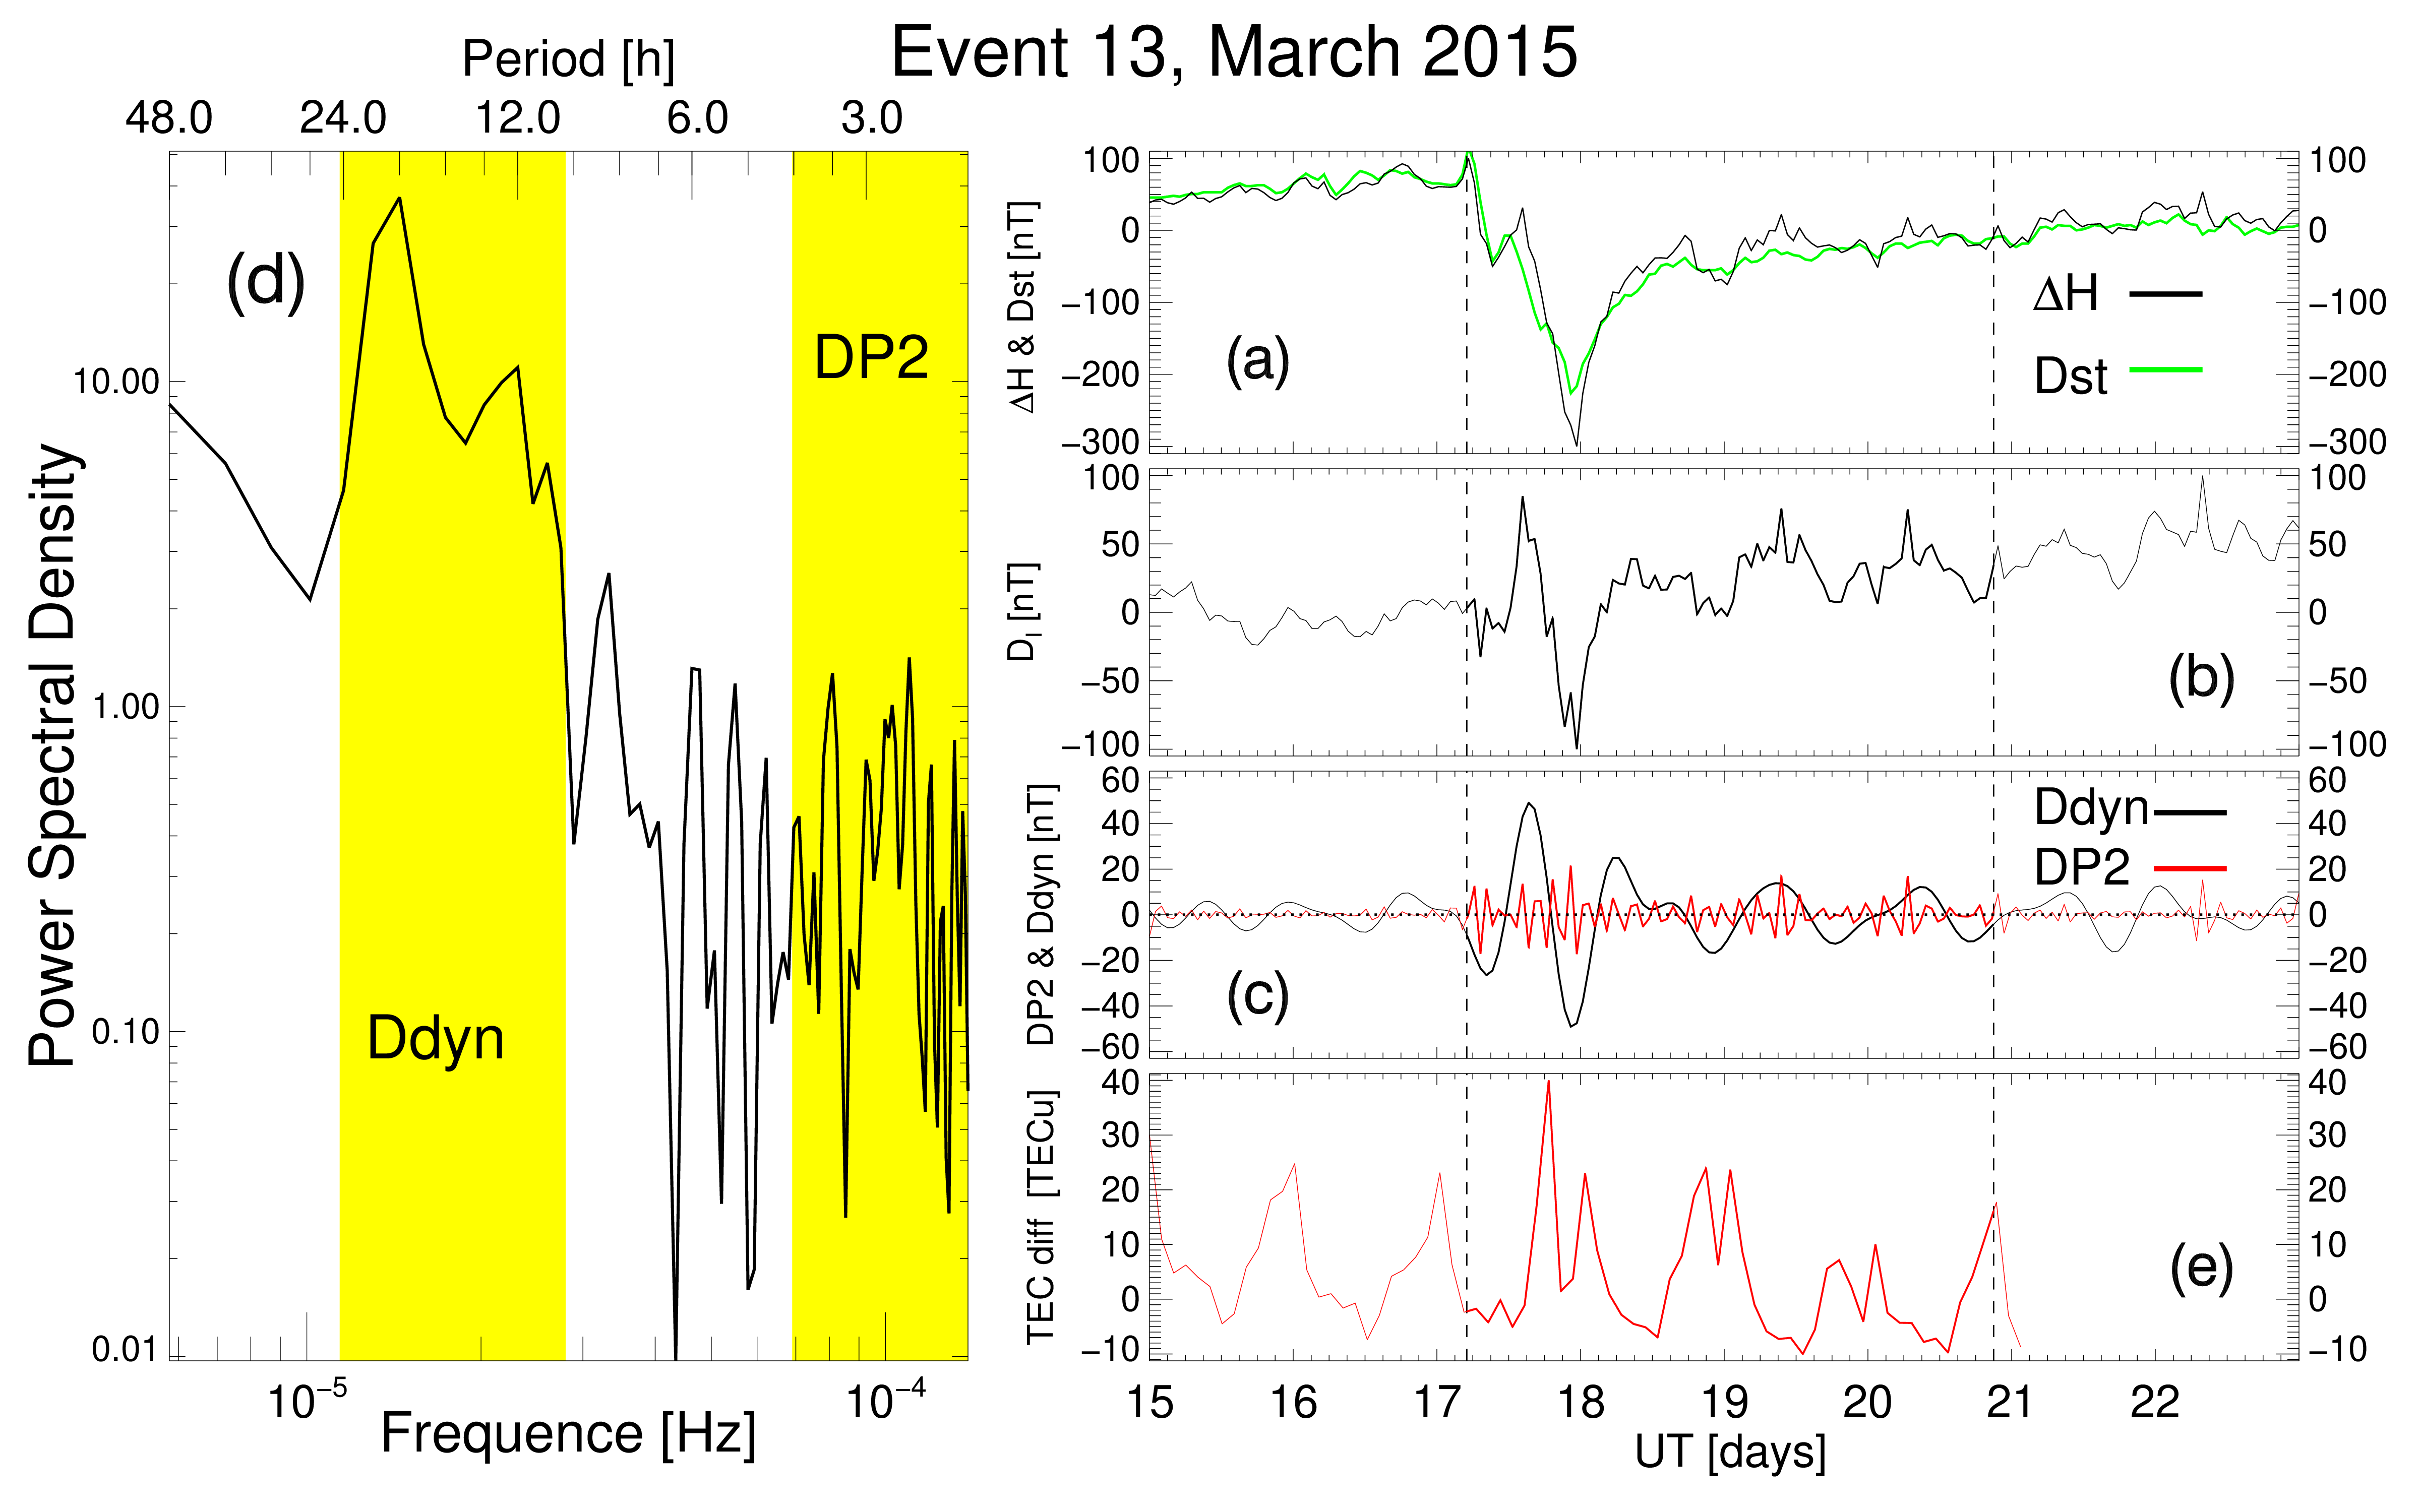
\includegraphics[width=0.85\textwidth]{Images/iono_PI_2015-03-15.png}
    \caption{Análisis del caso de estudio 13. Panel (a): $Dst$ (negro) y $\Delta H$ (verde). Panel (b): valor calculado de $D_I$. Panel (c): Perfiles reconstruidos de los efectos magnéticos de Ddyn (linea negra) y DP2 (linea roja). Panel (d): Espectro de Densidad de Potencia de $D_I$ o PSD. Panel (e): Medida de la diferencia de Contenido Total de Electrones (TEC) encima del centro de México. Las líneas verticales discontinuas indican el periodo de mayor impacto de la TG en el CTM. Las regiones amarillas en el panel (d) resaltan los anchos de bando asociados con  $Ddyn$ (25h - 10 h) y $DP2$ (menos de 4.5 h).}
    \label{fig:iono_resp}
\end{figure*}

En el panel (b) de la Figura \ref{fig:iono_resp}, se aprecia el resultado del perfil $D_I$ (Ecuación (\ref{eq:diono})), calculado a partir de las observaciones de TEO y los datos reportados del índice $Dst$. Subsecuentemente, se construyó un espectro de potencia \emph{PSD}. Para su construcción, tal y como se indica en la Sección \ref{psd_section} se utilizó una función ventana (Ventana de Hanning) para atenuar la dispersión de energía en los picos de potencia de interés. Las regiones de color amarillo resaltan los rangos de periodos (frecuencias), que son consistentes con los rangos de fluctuación del CMT regional debido a la presencia de \emph{Ddyn} y \emph{DP2}. En el panel se identifica el rango de frecuencias de \emph{Ddyn} al ajustar el periodo principal e identificar los picos de potencia. Es importante tomar en cuenta que, debido a la diferencia de los casos de estudio, pueden haber diferencias significativas en los rangos de \emph{Ddyn} para cada TG. Es por ello que los anchos de banda ajustados para cada TG pueden variar. 
\vspace{1 em}

En la Figura \ref{fig:iono_resp}(c) se presentan los perfiles de las perturbaciones ocasionadas por \emph{DP2} (linea roja) y \emph{Ddyn} (linea negra). Estos perfiles fueron construidos a partir de los rangos de frecuencias identificados a través de los procesos de filtros comentados en el párrafo anterior. Se puede observar que los incrementos de los efectos inducidos por \emph{Ddyn} y \emph{DP2} ocurren de forma simultanea con un incremento del $TEC_{dif}$ sobre el centro de México mostrado en el panel (e) de la Figura \ref{fig:iono_resp}, mencionado en la sección \ref{diono}. 
\vspace{1 em}

%El procedimiento previamente mostrado fue aplicado a los 20 casos de estudio usando datos de TEO. En las Figuras \ref{fig:iono_resp2} y \ref{fig:iono_resp3} del apéndice, se muestran los perfiles calculados de $D_I$, así como los perfiles de \emph{Ddyn} y \emph{DP2} de cada evento mostrado en la Tabla \ref{table1:GS_descp}. Al observar cada evento, se resaltan sus particularidades individuales, las cuales son evidentes en los perfiles de $D_I$ y sus perturbaciones magnéticas asociadas con \emph{Ddyn} y \emph{DP2}.
%\vspace{1 em}

A partir de las observaciones de los 20 eventos de la Tabla \ref{table1:GS_descp}, se encontró que generalmente, la amplitud de las oscilaciones magnéticas inducidas por \emph{Ddyn} son más intensas que aquellas inducidas por \emph{DP2}. Esto sugiere que, en la mayoría de los casos, los efectos de inducción magnética de \emph{Ddyn} son dominantes en el CMT local. Aunque también hay eventos para los cuales ambos efectos tienen intensidades similares. Se piensa en dos posibilidades para explicar estos resultados: El primero, es el mecanismo que desencadena la TG en sí, \emph{i.t.} y su reconexión magnética con el CMT. Esto puede afectar la evolución de la respuesta ionosférica, modificando directamente la evolución de las corrientes \emph{Ddyn} y \emph{DP2}. En segundo lugar, se debe considerar que los datos usados en un inicio tienen una resolución de 1h. En este caso, el muestreo de datos representa una limitación importante ya que las fluctuaciones magnéticas ocasionadas por \emph{DP2}, tal y como se menciona el \cite{nishida_68_fluctuations}, pueden tener periodos de menos de una hora hasta incluso unas poca decenas de minutos. En este escenario, es posible que se pierdan parte de las fluctuaciones más significativas inducidas por \emph{DP2}. Esto se puede resolver al usar datos del índice $SYM-H$ en vez de $Dst$, así como datos locales de 1 minuto de resolución, caso del cual se estará hablando en la sección \ref{PSD2}. 
\vspace{1 em}

\section{Validación de resultados} \label{validacion}

En la sección \ref{respuesta_dif}, identificamos diferencias substanciales entre la respuesta planetaria y la regional. En la sección \ref{resultados}, se determinaron los mecanismos geomagnéticos que tentativamente den origen a esas variaciones regionales, además de señalar su consistencia con la respuesta ionosférica medida mediante $TEC_{dif}$. Para validar estos resultados, se realizó una aproximación de múltiples pasos.  
\vspace{1 em}

Inicialmente, se aproximó el índice regional $\Delta H_{TEO}$ al definirlo como se muestra a continuación:

\begin{equation}
    \label{eq:deltaH}
    \Delta H_{TEO} = H_{TEO} - (H_{SQ} + H_0),
\end{equation}

Usando las ecuaciones (\ref{eq:diono}), (\ref{eq:diono_explicit}), y (\ref{eq:deltaH}), se deriva:

\begin{equation}
    \label{eq:deltaHandDst}
    \Delta H_{TEO} \approx Dst \cos(\lambda) + DP2 + Ddyn.
\end{equation}

Para simplificar, se denotó a $ Dst_\lambda$ como el efecto combinado de $ Dst\cos(\lambda)$, $DP2$, y $Ddyn$. Esto condujo al primer paso de validación, confirmando si el $ Dst_\lambda$ se aproximaba a $\Delta H$. Adicionalmente, se empleó a $ Dst_\lambda$ y los valores de $K_P$ para aproximar el valor local de $K$. 
\vspace{1 em}

La figura \ref{fig:iono_valid} muestra el proceso de validación aplicado para el evento 13. En el panel superior se observan sobrepuestos los perfiles de $\Delta H_{TEO}$ (negro), $Dst$ (verde), y $Dst_\lambda$ (rojo). Es evidente que, $Dst_\lambda$ consistentemente tiene un comportamiento más parecido a $\Delta H_{TEO}$ que $Dst$ , siendo esto válido para el periodo señalado por las lineas verticales discontinuas que enmarcan la fase principal y parte de la fase de recuperación de la TG. En el panel inferior se muestra que los valores $K$ planetarios (verde) y regionales (negro) difieren. Sin embargo, cuando $Dst_\lambda$ es combinado con $K_P$ usando las barras de incertidumbre, el perfil de $K$ local se ubica dentro de este rango.
\vspace{1 em}

\begin{figure}
\centering
    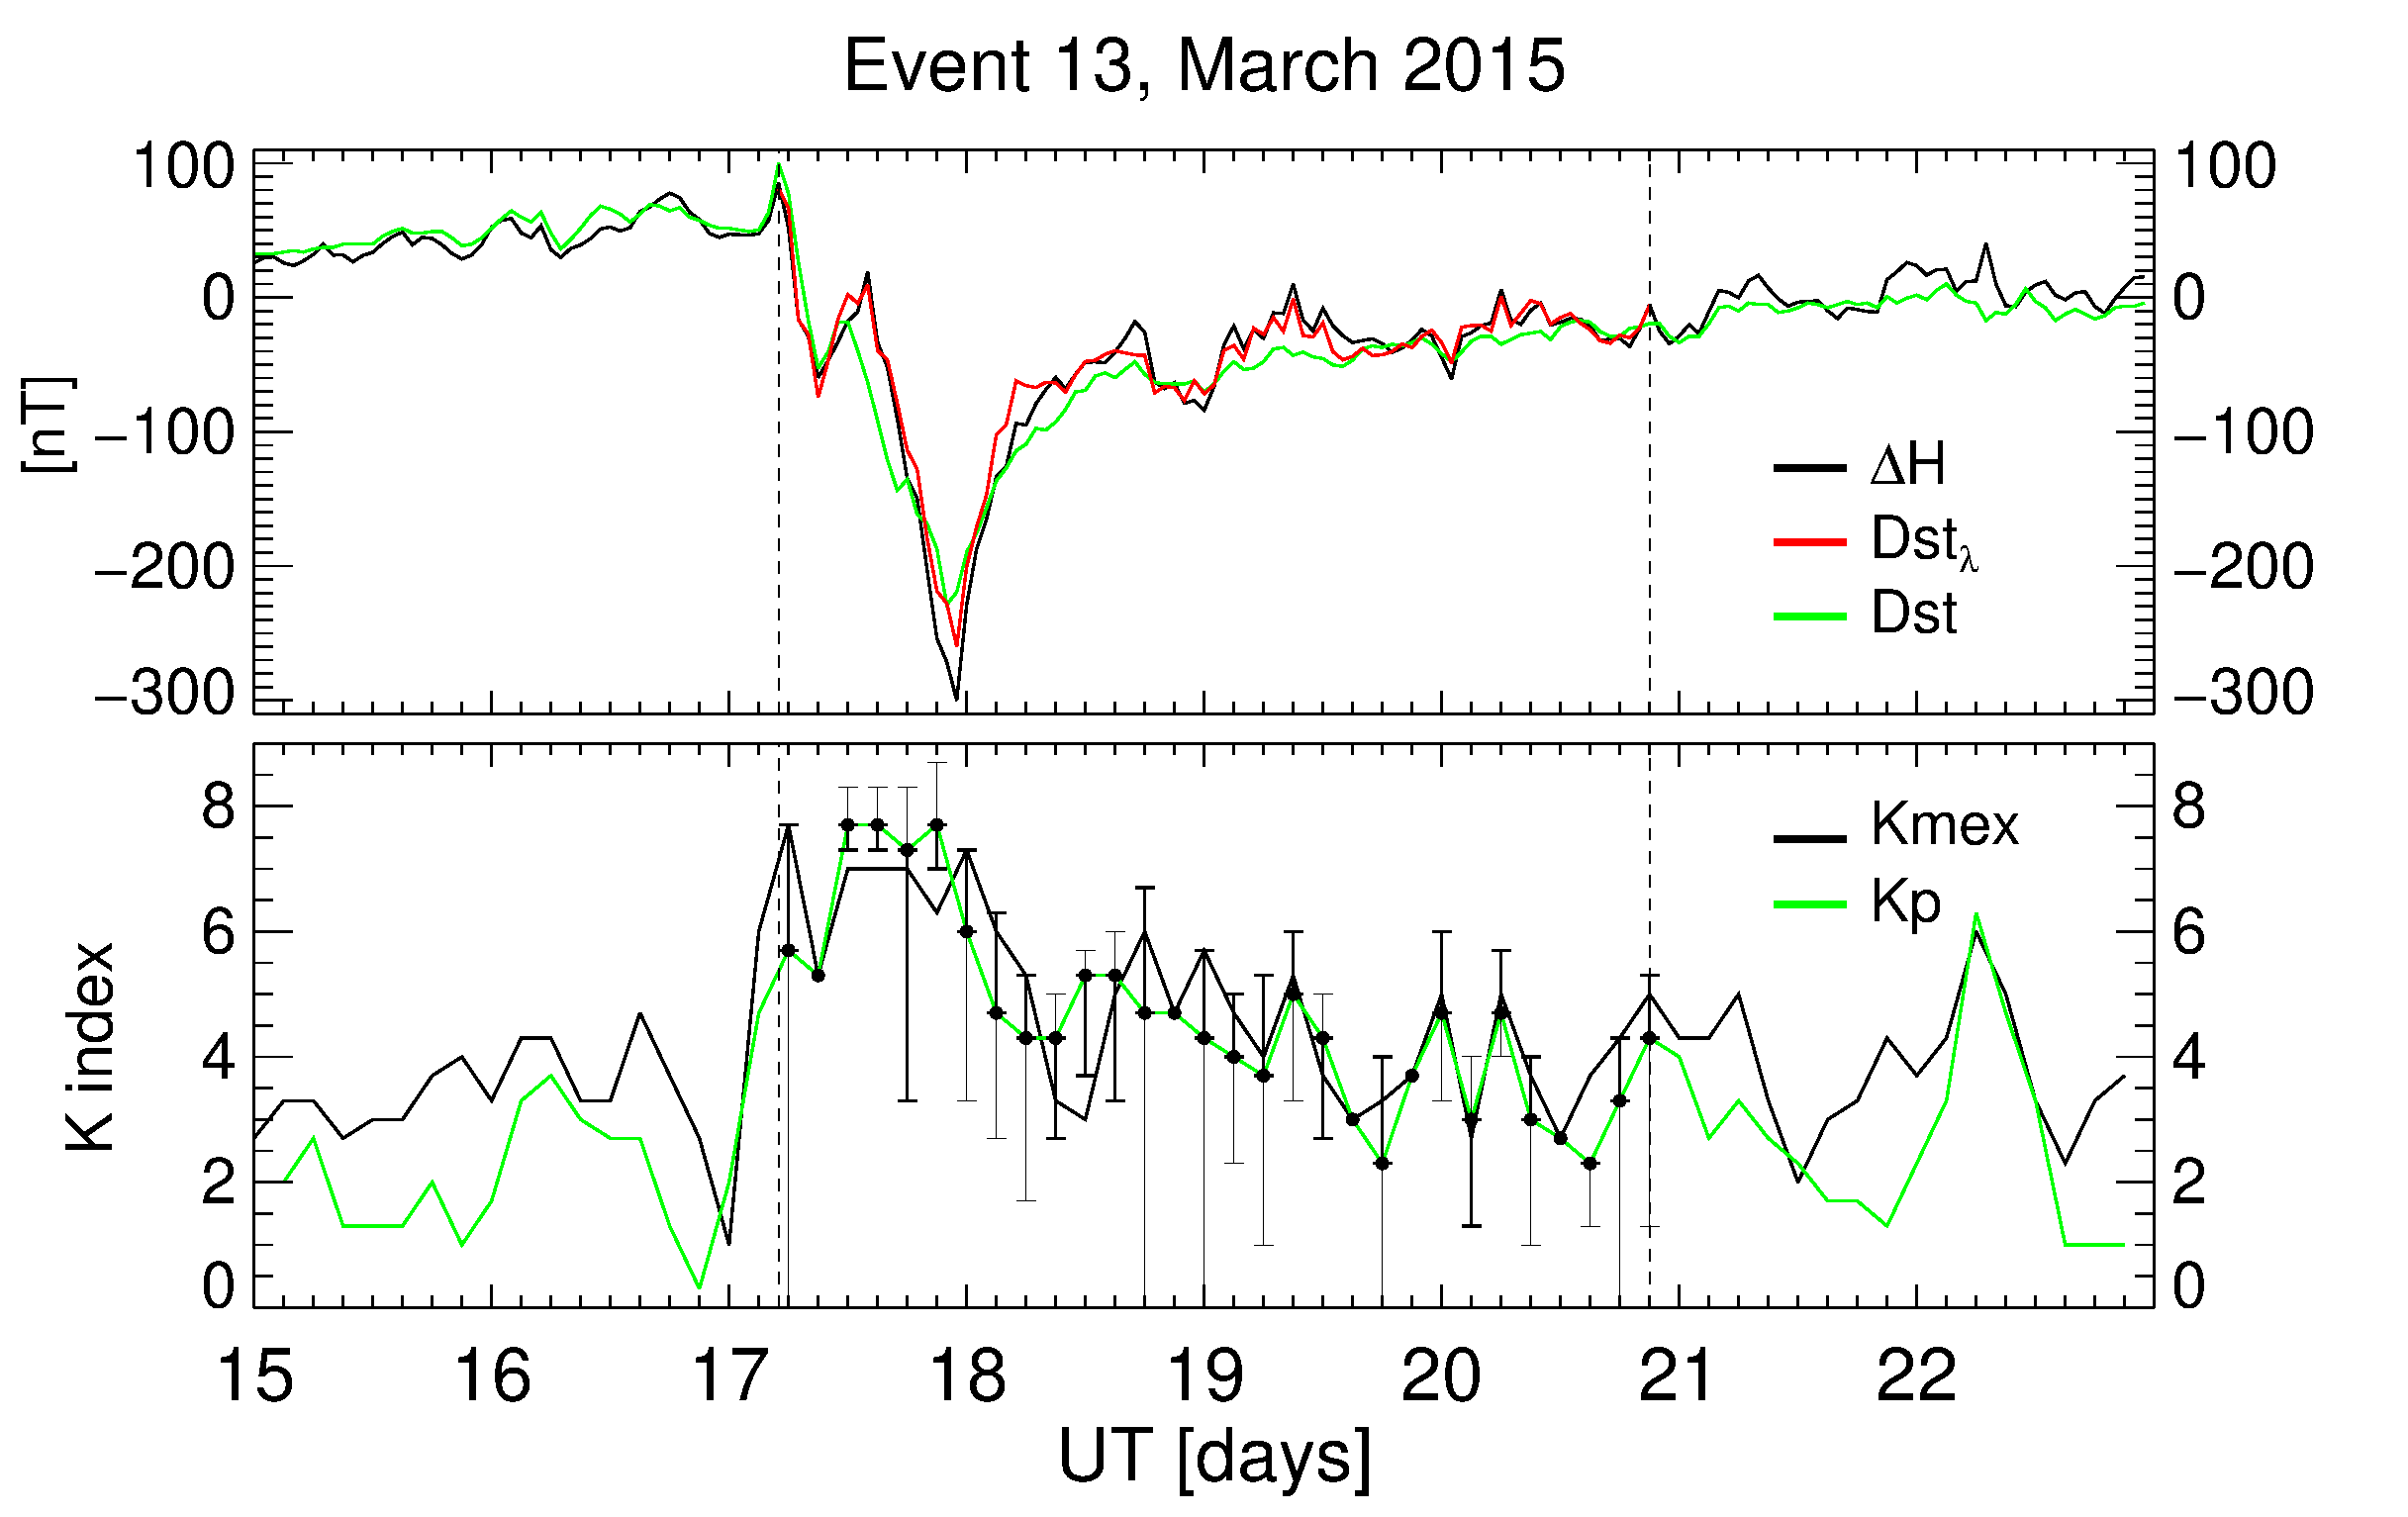
\includegraphics[width=0.7\textwidth]{Images/diono_valid_V4_2015-03-15.eps}
    \caption{Aproximación de los índices geomagnéticos  $\Delta H_{TEO}$ (arriba) y el $K_{TEO}$ (abajo). Las lineas verdes representan los índices planetarios mientras que las líneas negras representan los índices locales. El índice aproximado $\Delta H_{TEO}$ es representado mediante la linea roja, mientras que las barras de error representan un rango de aproximación para el índice $K_{TEO}$.}
    \label{fig:iono_valid}
\end{figure}

Para  validar de forma comprensiva, este proceso es aplicado a todos los casos de estudio. Consistentemente, $ Dst_\lambda$ se aproxima a $\Delta H_{TEO}$; mientras que $K_p$ combinado con los efectos de $Dst_\lambda$ envuelve los valores regionales de $K_{TEO}$.
\vspace{1 em}

Adicionalmente, se condujo un método cuantitativo de comparación. Se calculó el error promedio absoluto de la diferencia entre $\Delta H_{TEO}$-$Dst$ y $\Delta H$-$Dst_\lambda$ [nT]. Como se ilustra en la Figura \ref{fig:valid}

\begin{figure}
\centering
    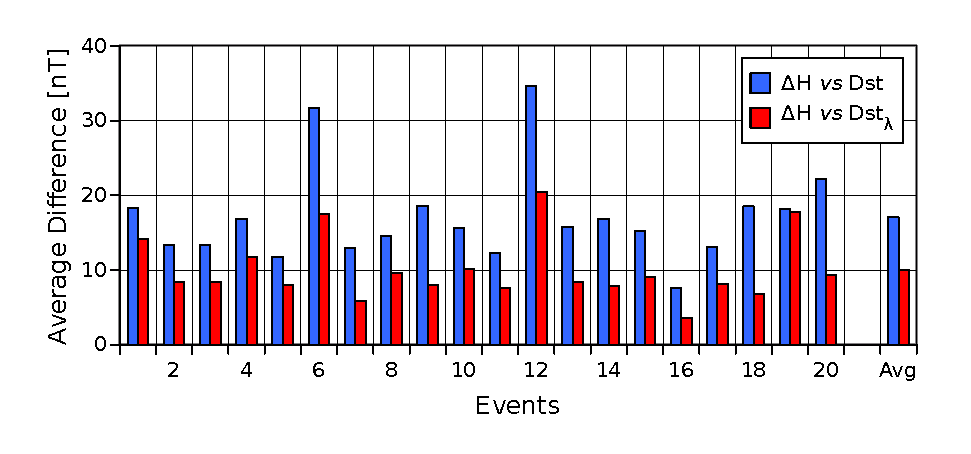
\includegraphics[width=0.7\textwidth]{Images/prom_dist.eps}
    \caption{Error promedio medido en nT entre $\Delta$H vs Dst (barras azules) y $\Delta$H vs $Dst_\lambda$ (barras rojas).}
    \label{fig:valid}
\end{figure}

En la figura \ref{fig:valid} se puede observar que el promedio absoluto del error entre $\Delta H_{TEO}$-$Dst_\lambda$ es menor que $\Delta H_{TEO}$-$Dst$. Esto indica un comportamiento más parecido por parte de $Dst_\lambda$ con respecto de la respuesta geomagnética regional observada. 
\vspace{1 em}

El paso final involucra resaltar la gráfica de dispersión de la Figura \ref{fig:disp}, empleando a $Dst_\lambda$ en vez de $Dst$. El resultado se muestra en la Figura \ref{fig:valid_disp2} , los datos puntuales (diamantes) más cercanos a la identidad (linea negra), en contraste con la Figura \ref{fig:disp}. Más aún, $R^2$ tiene un incremento de 0.77 a 0.86 para el rango de $Dst \ge -100\, {\rm nT}$, mientras que para el rango de $Dst < -100\, {\rm nT}$, $R^2$ tiene un aumento significativo de 0.75, con respecto a su valor original ($R^2=0.42$).
\vspace{1 em}

\begin{figure}
    \centering
     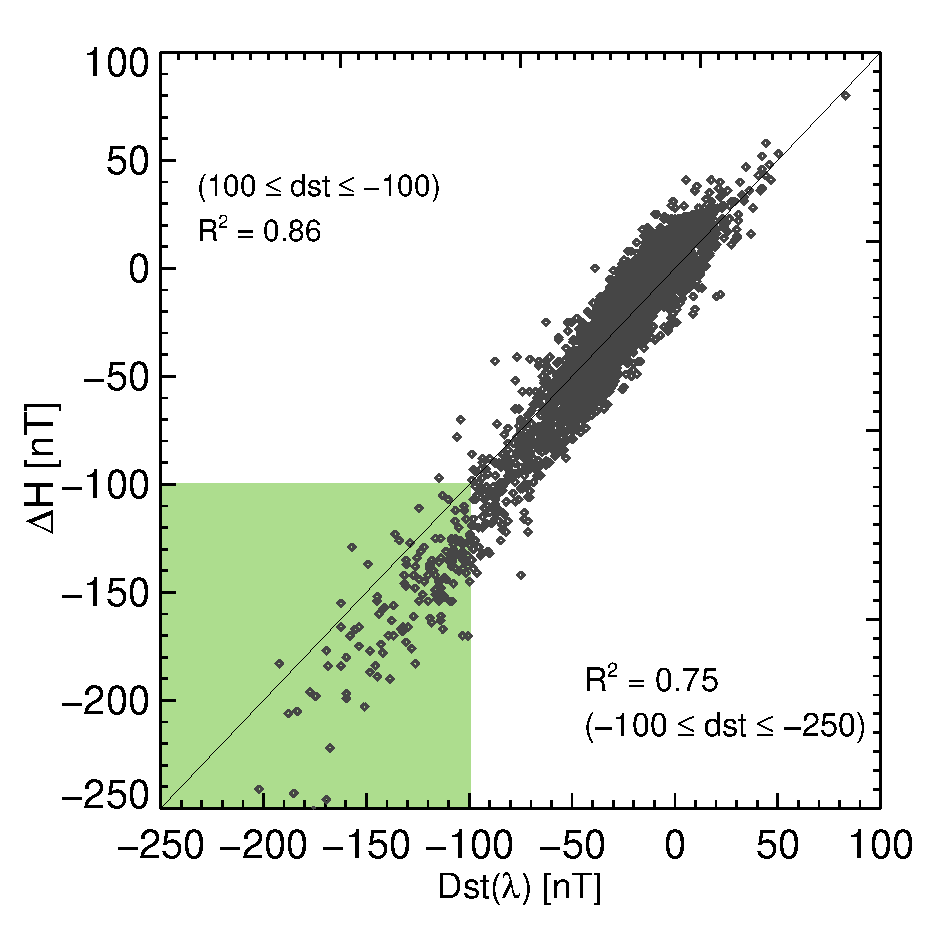
\includegraphics[width=0.7\textwidth]{Images/dispersion_general_dst_ld.eps}
      \caption{Gráfica de dispersión $\Delta H_{TEO}$ (eje vertical) con respecto a $Dst_\lambda$ (eje horizontal) para todos los eventos TG. La región verde representa un umbral de -100 nT en que fue calculado el segundo $R^2$.}
       \label{fig:valid_disp2}
\end{figure}

Con el proceso de validación, se demostró que las perturbaciones magnéticas potencialmente inducidas por las corrientes ionosféricas $DP2$ y $Ddyn$, cuando se combinan con la respuesta planetaria (índice $Dst$) permiten una aproximación cuantitativa aceptable de la respuesta geomagnética regional. Más aún, las diferencias entre los datos regionales y planetarios se reducen de forma sustancial al integrar los efectos magnéticos de $DP2$ y $Ddyn$ en la respuesta planetaria.
\vspace{1 em}

\section{Análisis de espectral II}
\label{PSD2}

\subsection{Potencia espectral, resolución: 1 min}

Con el uso de datos con resolución de 1 minuto, el primer paso fue el de realizar un estudio más detallado de los PSD. En la Figura \ref{fig:powerlaw} se muestra el PSD aplicado para el evento 21, ocurrido en 2023 y para el cual se utilizan datos de COE. En el panel de arriba se muestra la serie de tiempo, una vez removidos los efectos $H_{SQ}$, mientras que en el panel inferior se observa la misma serie de tiempo sin remover $H_{SQ}$.
\vspace{1 em}

Una de las primeras observaciones es que, independientemente del panel (o del evento en cuestión), en ambos casos se muestra lo que parece ser dos leyes de potencia, asociadas a los rangos de frecuencia en que se presentan las fluctuaciones inducidas por \emph{Ddyn} y \emph{DP2}. En la Figura las leyes de potencia se representan mediante las lineas rojas continuas que se denominaron como $a1$ y $a2$. Las leyes de potencia fueron calculadas a partir de mínimos cuadrados, de acuerdo al criterio utilizado por \cite{LS_red_noise}. El par de lineas segmentadas señala el error de la ley de potencia. Cabe señalar que, $a1$ y $a2$ se ven afectadas por la presencia del efecto $H_{SQ}$, pues en la Figura \ref{fig:powerlaw}, la integración del efecto $H_{SQ}$ provoca un desajuste con respecto de la \emph{PSD}. Otra consideración a tomar en cuenta es que las leyes de potencia calculadas también se ven altamente afectadas por los picos negativos, en determinados eventos.
\vspace{1 em}

 
Se puede observar un fenómeno interesante entre $a1$ y $a2$ (en la banda de periodo de entre las 6h y las 3 h) un fenómeno recurrente en los eventos. Es la presencia de lo que parece ser, un efecto escalón, donde entre cada ley de potencia pareciera presentarse otra potencia. De igual forma, para fluctuaciones de periodo menor a 20 minutos, se observa en general otra ley de potencia más, la cual pareciera estar más cercana al ruido blanco. En general, diferentes leyes de potencia en un PSD son un indicativo de fluctuaciones persistentes, por lo que se espera conseguir información de interés asociado a las leyes de potencia presentes en cada PSD.
\vspace{1 em}

\begin{figure}
    \centering
     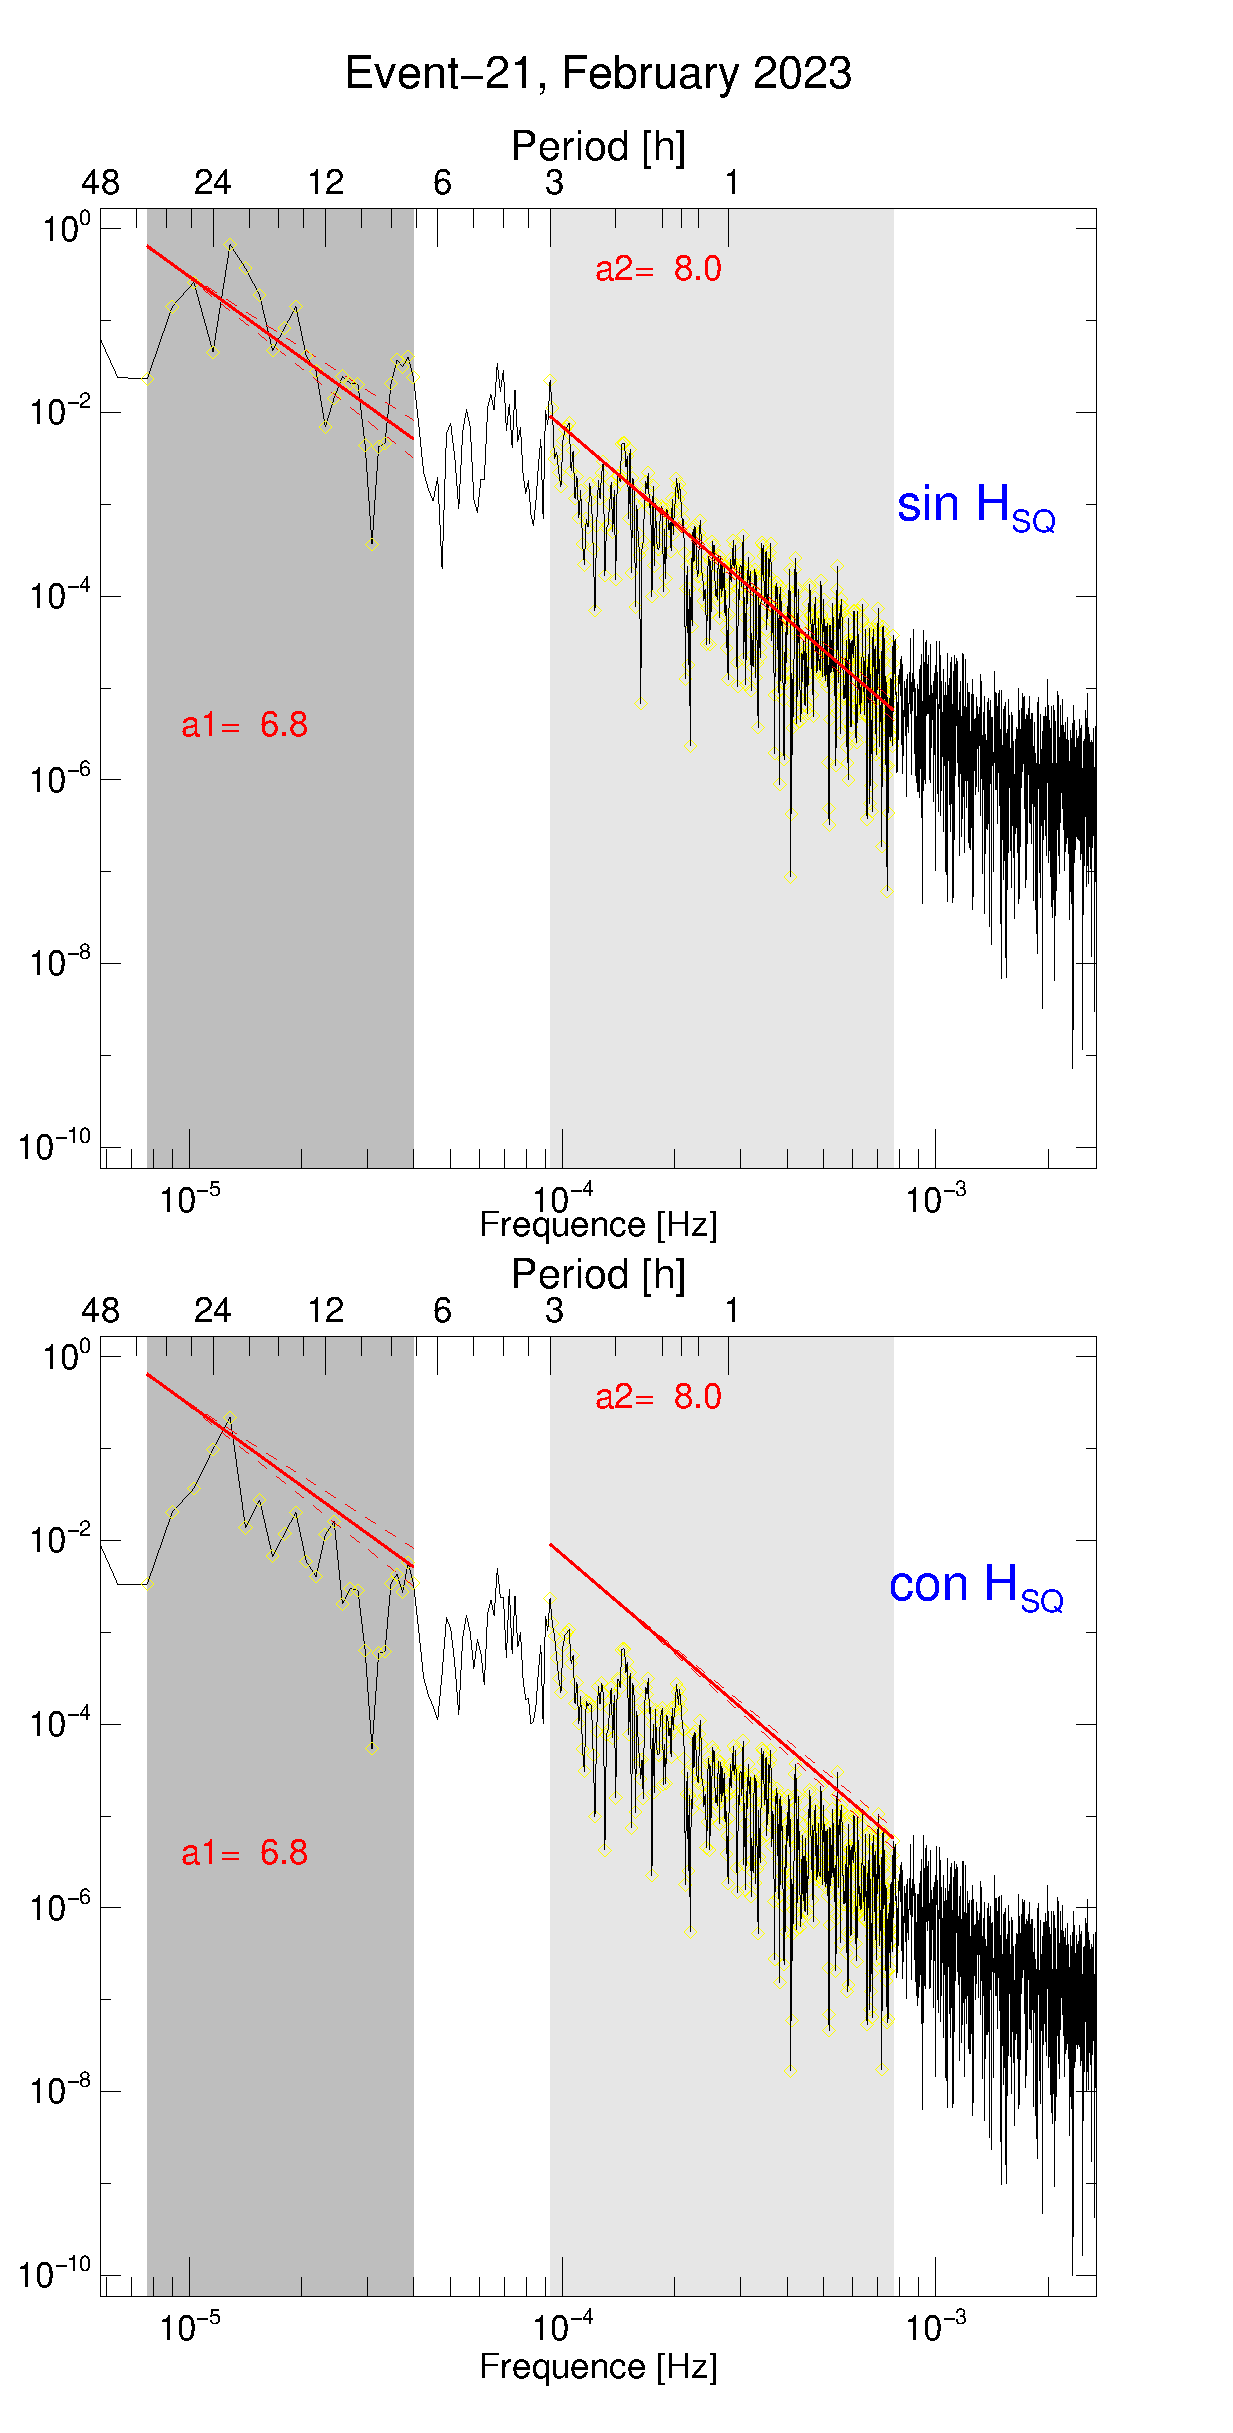
\includegraphics[width=0.7\textwidth]{Images/cap3/powerlaw/diono_PWS_powerL_2023-02-25.eps}
      \caption{Espectro de potencia (linea negra), considerando para la serie de tiempo removiendo el efecto $H_{SQ}$ (arriba) y sin removerlo (abajo). Las líneas rojas representan las leyes de potencia asociadas con \emph{Ddyn} (a1) y \emph{DP2} (a2). Las regiones gris oscuro y gris claro resaltan los anchos de banda que abarcan estas leyes de potencia.}
       \label{fig:powerlaw}
\end{figure}


\subsection{Análisis de ondículas}

A partir del trabajo realizado por \cite{2021amory}, donde se concluyó que un análisis de ondículas sería más adecuado para este tipo de fenómenos, se optó por hacer lo propio para los 23 eventos en México. En este caso se utilizó la ondícula de Morlet como ondícula madre. En la Figura \ref{fig:wave} se muestra el resultado de aplicar un análisis de ondícula, mientras que en la Figura \ref{fig:wavepower} se muestra la potencia espectral de la ondícula. La malla que se observa en ambas figuras es la región afectada por el efecto borde, o Cono de Influencia. 
\vspace{1 em}

Se observa en la Figura \ref{fig:wave} un efecto consistente en periodos de entre 28h y 12h con la presencia de una TG entre el 26 de febrero y el 4 de marzo del 2023. Los tonos cálidos y fríos son consistentes con los periodos de día y noche, los cuales son importantes en el fenómeno de \emph{Ddyn}. Además, se puede observar los días en que éste fenómeno tuvo una mayor amplitud. Por otro lado, se observan fluctuaciones en el rango de las 4h hasta menos de 1h, los cuales se limitan a aquellos periodos donde se presenta una reconexión magnética, lo cual es consistente con el fenómeno \emph{DP2}. 
\vspace{1 em}

En algunos casos (eventos 4, 5, 6, 13, 15, 19) se observó un efecto persistente de periodo entorno a las 48h - 72h. Esto también fue observado en los PSD de los respectivos eventos. Una primera hipótesis planteada sería un efecto no suficientemente bien atenuado de la línea base día a día. Sin embargo, este rango entra dentro del Cono de Influencia, por lo que no debería ser tomado en cuenta.  
\vspace{1 em}

En esos mismos eventos, también se observa una potencia en la banda de frecuencias asociada con \emph{Ddyn}. Esto en principio podría indicar que durante los eventos 4, 5, 6, 13, 15, 19; el efecto magnético inducido por \emph{Ddyn} no fue muy significativo dentro de las variaciones magnéticas locales. 
\vspace{1 em}



\begin{figure}
    \centering
     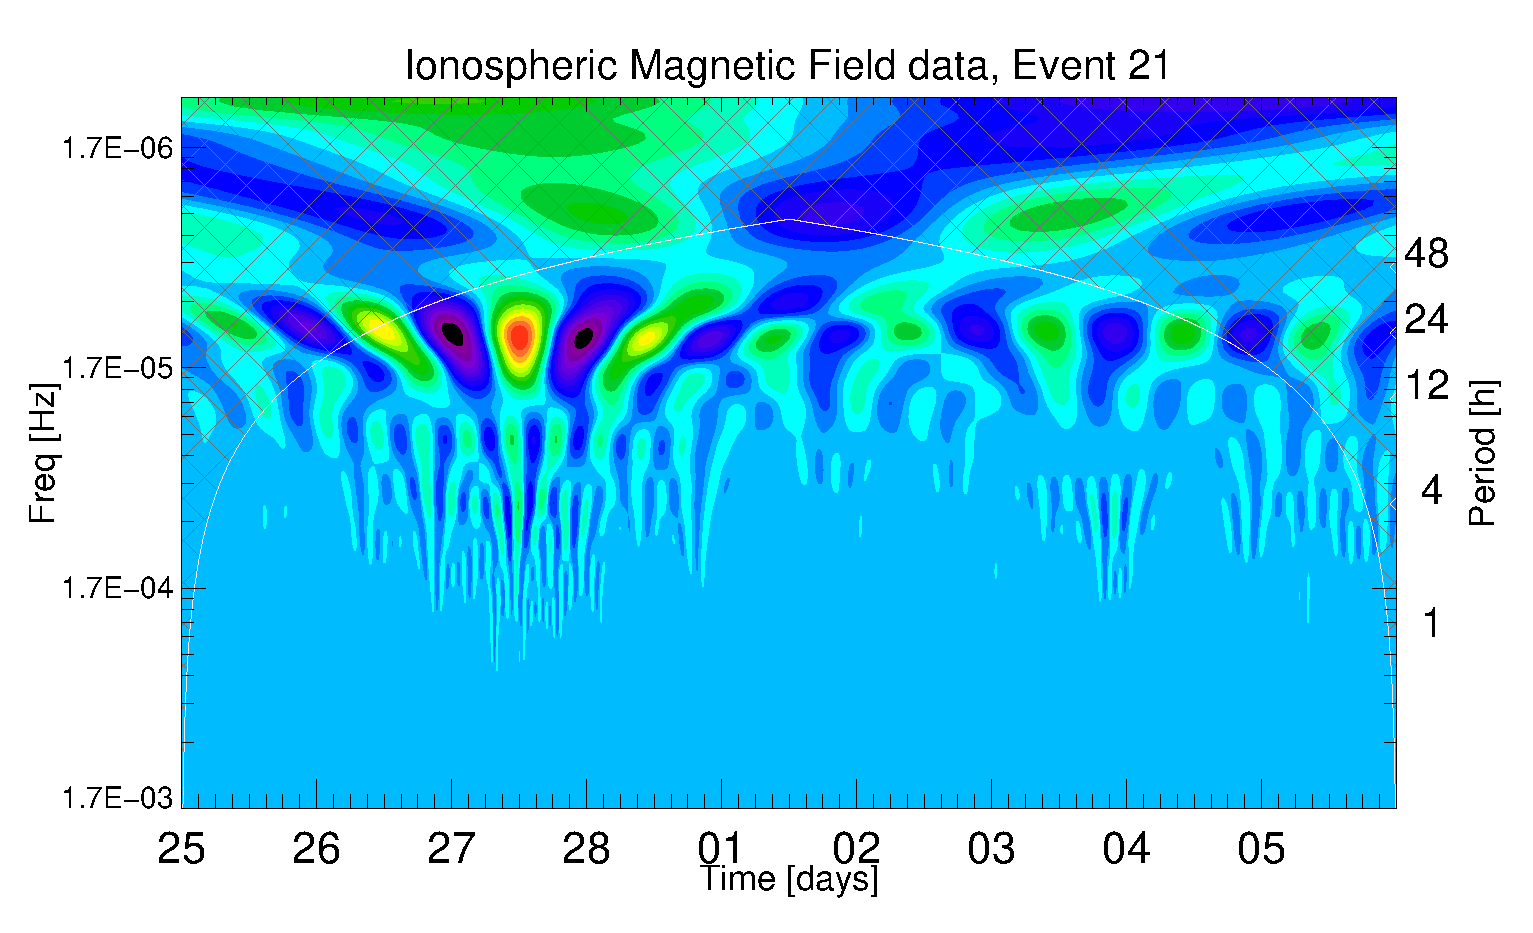
\includegraphics[width=0.7\textwidth]{Images/cap2/wave/wave_2023-02-25.uncut.eps}
      \caption{Análisis de ondícula aplicado a la TG 21. El mayado en la parte superior representa el Cono de influencia ocasionado por el efecto de borde.}
       \label{fig:wave}
\end{figure}

Por otro lado, también se calculó la potencia espectral de la ondícula, lo cual se ve plasmado en la Figura \ref{fig:wavepower}. En la Figura se observa claramente los días en que \emph{Ddyn} tuvo un mayor impacto en el CMT local. Por otro lado, no se observan fluctuaciones relevantes en el rango de fluctuación de \emph{DP2}.
\vspace{1 em}

Por último, algo que es necesario observar en este evento y que también fue observado en los eventos 1, 3, 11, 18 y 23 es la presencia de aparentes armónicos, potencialmente asociados con \emph{Ddyn}. Este y otros aspectos serán investigados posteriormente.


\begin{figure}
    \centering
     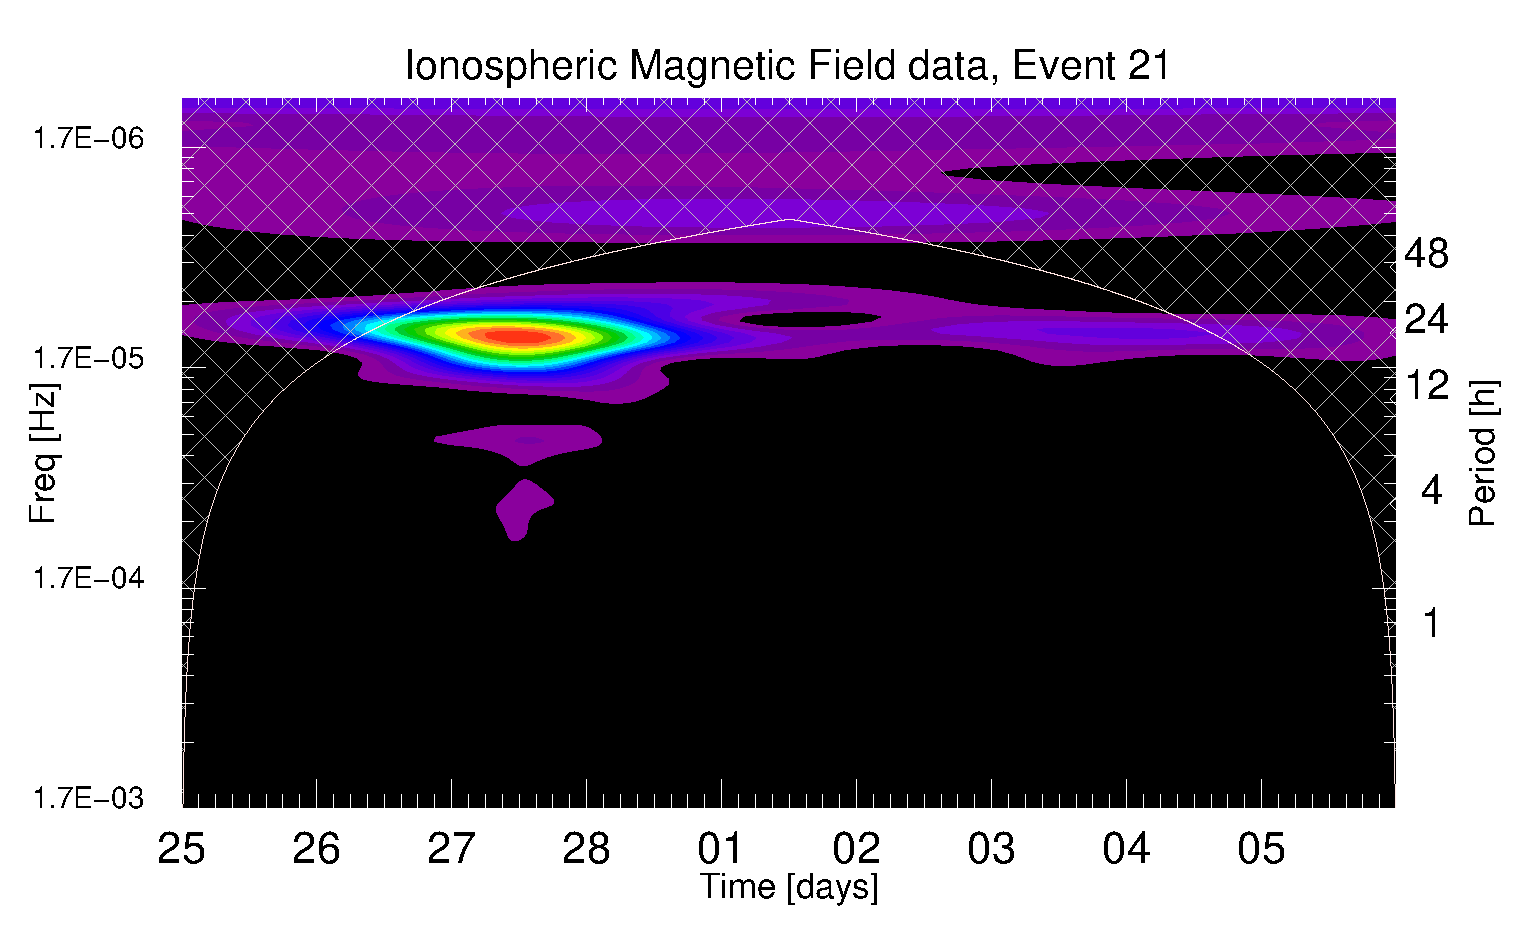
\includegraphics[width=0.7\textwidth]{Images/cap2/power/power_2023-02-25.uncut.eps}
      \caption{Análisis de potencia y significancia de ondícula, aplicado a la TG 21. El mayado en la parte superior representa el Cono de influencia ocasionado por el efecto de borde.}
       \label{fig:wavepower}
\end{figure}

\section{Observaciones finales}
En este primer trabajo, se estudiaron las manifestaciones regionales de clima espacial. El enfoque fueron las diferencias en la respuesta geomagnética regional con respecto a la planetaria durante periodos de Tormentas Geomagnéticas (TG) intensas sobre el centro de México. También se investigaron los mecanismos físicos responsables de tales variaciones geomagnéticas. Se utilizaron los registros geomagnéticos del observatorio geomagnético de Teoloyucan (TEO), localizado al norte de la Ciudad de México. También se están empleando datos de la estación geomagnética de Coeneo (COE), localizada en Michoacán. También se utilizaron los datos de los índices planetarios $Dst$ y $K_P$, los índices regionales $\Delta H_{TEO}$ y $\Delta H_{COE}$, así como el Contenido Total de Electrones, proporcionado por el Laboratorio Nacional de Clima Espacial (LANCE).
\vspace{1 em}

Se seleccionaron en principio 20 casos de estudio (véase la Tabla \ref{table1:GS_descp}) para el caso de los datos de TEO, más 3 casos (Tabla \ref{table2:GS_descp}) con datos de COE. Para todos los casos de estudio, se identificó la evidencia de una respuesta geomagnética regional relevante a través de la gráfica de dispersión (Véase la Figura \ref{fig:disp}). En este caso, se encontró que en el rango de $Dst < -100 {\rm nT}$, hay una tendencia para el índice geomagnético regional a desviarse del planetario. Se asume este comportamiento como evidencia de una respuesta geomagnética regional.
\vspace{1 em}

Subsecuentemente, se validaron las contribuciones geomagnéticas debidas a las corrientes $Ddyn$ y $DP2$. Primero, se aproximó la respuesta regional ($\Delta H_{TEO}$ y $K_{TEO}$) a partir de combinar $K_P$ y $Dst$ con los efectos geomagnéticos inducidos por $Ddyn$ y $DP2$. Posteriormente, se calculó la diferencia (o error) entre $\Delta H_{TEO}$ y $Dst$, con y sin considerar los efectos de las corrientes ionosféricas. Finalmente, se analizaron los efectos de dispersión entre $\Delta H_{TEO}$ y $Dst$, combinando éste último con los efectos magnéticos de $Ddyn$ y $DP2$. Para todos los casos, se encontró que la respuesta geomagnética planetaria combinada con las perturbaciones geomagnéticas inducidas por las corrientes $Ddyn$ y $DP2$ permitía una aproximación aceptable (cuantitativa y cualitativamente).
\vspace{1 em}

En una etapa más reciente del estudio, se utilizaron datos magnéticos locales con resolución de 1 minuto, así como el índice planetario $SYM-H$. En el segundo estudio de \emph{PSD} se observó un fenómeno recurrente: la presencia de múltiples leyes de potencias, asociadas con las bandas de frecuencia en que \emph{Ddyn} y \emph{DP2} inducen perturbaciones magnéticas a las cuales denominamos como $a1$ y a2. Éste fenómeno se observó inclusive en aquellos eventos donde los picos de potencia \emph{Ddyn} no eran muy significativos (eventos 4, 5, 6, 13, 15, 19). También se observó una tercera ley de potencia, intermedia, entre $a1$ y $a2$, cuya banda no está asociada a ninguna de las corrientes \emph{Ddyn} ni \emph{DP2}. Una primera hipótesis indica que pudiera tratarse de un efecto de armónico producido por \emph{Ddyn}.
\vspace{1 em}

Se realizó un análisis de ondículas donde se estudió el efecto magnético asociado con \emph{Ddyn} y \emph{DP2} y cómo éste se presentaba en el dominio del tiempo y de frecuencias. Se pudo observar que la banda de frecuencia en que se presenta el efecto magnético de \emph{Ddyn} es consistente con lo observado en los estudios de \emph{Ddyn}, teniendo periodos mínimos de entre 12h y 10h en algunos casos. Esto es importante considerar, ya que muchos autores como \cite{amory2020_filtros, ionos1} consideran el ajuste de filtros pasa-bandas para periodos mínimos de 18h. Por otro lado, de forma consistente con lo observado en los \emph{PSD}, no se observaron potencias significativas asociadas a las fluctuaciones inducidas por \emph{Ddyn} en los eventos ya mencionados. En esos mismos eventos se observaron potencias siginicativas entorno a las 72h-48h. Estas oscilaciones están por encima de las 36h, máximo periodo de oscilación para \emph{Ddyn} manejado por algunos autores por lo que no podría considerarse en principio como parte de este fenómeno. Una posible hipótesis que explica este fenómeno sería un persistente efecto de variación día a día que no fue del todo atenuado durante el pre-procesado de datos. No obstante, éstas oscilaciones entran dentro del rango del Cono de Influencia, por lo que no deben ser tomadas en cuenta. 
\vspace{1 em}

Por último, se destaca que a partir de la primera etapa de este trabajo de investigación que abarca el análisis de los primeros 20 casos hasta la sección \ref{validacion}, se realizó un primer artículo de investigación. Éste artículo actualmente se encuentra bajo revisión en la \textit{Journal of Atmospheric and Solar-Terrestrial Physics}, perteneciente a la editorial \textit{Elsevier}. 


